\documentclass[border=6pt]{standalone}
\usepackage{tikz}
\usetikzlibrary{arrows.meta,calc,decorations.pathreplacing,positioning}
\begin{document}

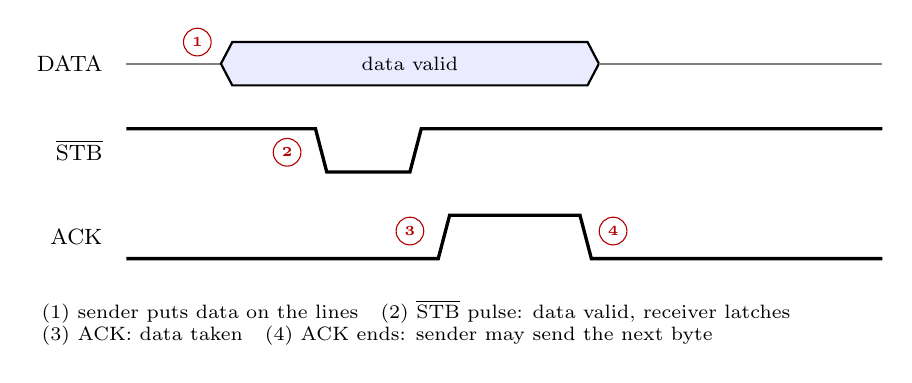
\begin{tikzpicture}[>=Stealth,font=\small,x=1.2cm,y=1cm]
% row 0 y=0
\node[anchor=east,font=\footnotesize,align=right] at (-0.15,0.275) {DATA};
\draw[thick,gray] (0,0.275) -- (1,0.275);
\draw[thick,fill=blue!8] (1,0.275) -- (1.12,0.55) -- (4.88,0.55) -- (5,0.275) -- (4.88,0) -- (1.12,0) -- cycle;
\node[font=\scriptsize] at (3,0.275) {data valid};
\draw[thick,gray] (5,0.275) -- (8,0.275);
% row 1 y=-1.1
\node[anchor=east,font=\footnotesize,align=right] at (-0.15,-0.825) {$\overline{\mathrm{STB}}$};
\draw[very thick] (0,-0.55) -- (2,-0.55) -- (2.12,-1.1) -- (3,-1.1) -- (3.12,-0.55) -- (8,-0.55);
% row 2 y=-2.2
\node[anchor=east,font=\footnotesize,align=right] at (-0.15,-1.925) {ACK};
\draw[very thick] (0,-2.2) -- (3.3,-2.2) -- (3.42,-1.65) -- (4.8,-1.65) -- (4.92,-2.2) -- (8,-2.2);
\tikzset{n/.style={circle,draw=red!70!black,font=\tiny\bfseries,text=red!70!black,inner sep=0.5pt,minimum size=10pt}}
\node[n] at (0.75,0.55) {1};\node[n] at (1.7,-0.85) {2};\node[n] at (3.0,-1.85) {3};\node[n] at (5.15,-1.85) {4};
\node[font=\scriptsize,anchor=north west,align=left] at (-1.0,-2.6) {(1) sender puts data on the lines\quad (2) $\overline{\mathrm{STB}}$ pulse: data valid, receiver latches\\(3) ACK: data taken\quad (4) ACK ends: sender may send the next byte};
\end{tikzpicture}
\end{document}
